\section{Kontextdiagramm}

\begin{tcolorbox}[title=Kontextdiagramm]
    \textbf{Kontextdiagramme} liefern eine grafische Übersicht einzelner Systeme in ihrem Kontext.\\
    \noindent
    In einem  \textbf{Kontextdiagramm} werden diese Systeme ohne ihre innere Struktur dargestellt\footnote{
        diese können bspw. in einem Feinentwurf bei der Entwicklung der Architektur festgelegt werden
    }.\\
    Kontextdiagramme zeigen außerdem Schnittstellen der Systeme zu anderen Systemen oder Anwendern sowie die wichtigsten Anwendungsfälle.\\
    Als Notation für Kontextdiagramme werden i.d.R. \textbf{UML Use Case-Diagramme} benutzt, wobei Systeme als Pakete dargestellt werden, bei denen ihr Datenfluss durch Pfeile mit Richtungsangaben dargestellt wird (s. Abbildung~\ref{fig:contextdiagram_cc}).
\end{tcolorbox}


\begin{figure}
    \centering
    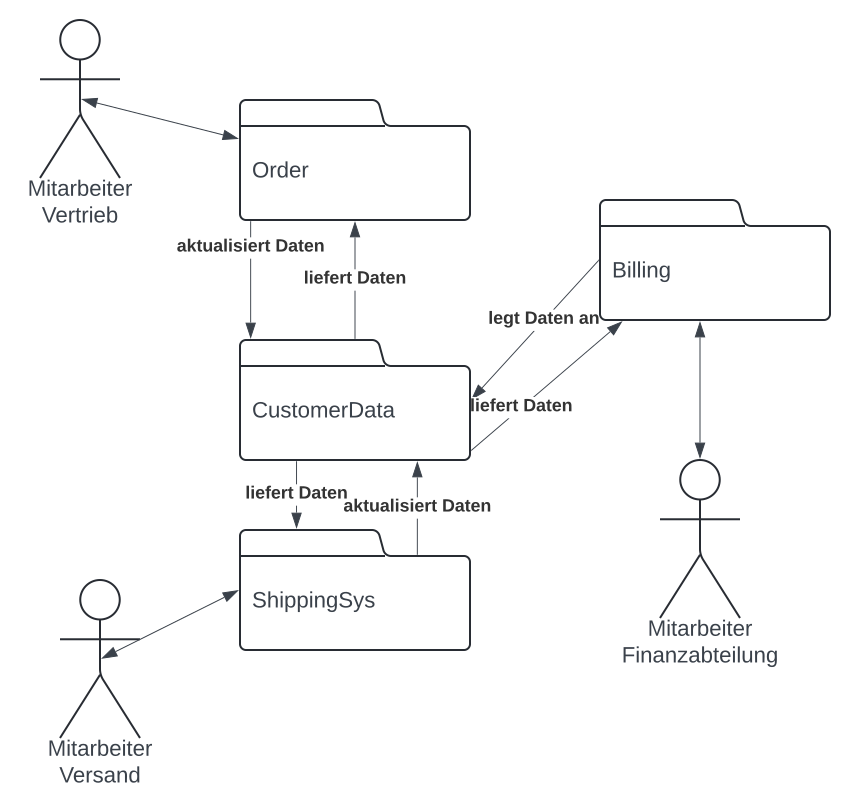
\includegraphics[scale=0.4]{chapters/Anhang/CheatSheets/img/contextdiagram}
    \caption{Beispiel für ein Kontextdiagramm. (Quelle: eigene)}
    \label{fig:contextdiagram_cc}
\end{figure}
